Il \textit{Data Analyzer} si occupa dell'analisi dei dati raccolti dal \textit{Data Collector} al fine di generale gli allarmi che saranno poi visibili agli utenti tramite l'applicazione client. Come per il \textit{Data Collector}, si è deciso di implementare questo componente come un applicativo Python che verrà in seguito distribuito su un Raspberry Pi4 per la sua esecuzione periodica. Si è scelto di utilizzare questo linguaggio di programmazione poiché sono disponibili numerose librerie per effettuare analisi dei dati, moduli e package che verranno sfruttati per la generazione delle allerte. In particolare, si è scelto di implementare queste ultime per segnalare i rischi nebbia o brina e l'imminente arrivo di una forte perturbazione. Nella figura \ref{fig:DAFlowChart} è rappresentato il diagramma di flusso relativo al Data Analyzer. All'avvio dell'applicazione vengono inizializzate alcune strutture dati di supporto all'esecuzione ciclica degli algoritmi per l'analisi dei dati, algoritmi che sono descritti dettagliatamente in seguito. Successivamente, viene eseguito un tentativo di connessione con il DB seguendo una strategia uguale a quella utilizzata per il \textit{Data Collector}. Se la connessione viene stabilita, allora vengono recuperati dal DB e memorizzati i codici identificativi delle stazioni meteorologiche; essi saranno utilizzati successivamente per accedere ai dati da fornire in input agli algoritmi per la generazione degli allarmi. Dopodiché, viene avviato un thread per ogni zona, il quale si occuperà della generazione delle allerte maltempo tramite l'analisi dei dati relativi alla pressione atmosferica. Altresì vengono avviati i thread che si occupano di analizzare i dati di temperatura e umidità relativa al fine di creare le allerte nebbia e brina. Infine, si attende la terminazione di tutti i thread precedentemente avviati e, a join concluso, viene chiusa la connessione con il DB. Da notare che la periodicità del ciclo è di 5 minuti.

\begin{figure}[h!]
	\centering
	\includegraphics[height=590px]{./Iterazione 3/OtherFiles/FC - Data analyzer}
	\caption{diagramma di flusso relativo all'esecuzione del componente Data Analyzer.}
	\label{fig:DAFlowChart}
\end{figure}

\clearpage

\paragraph{Generatore di allerte maltempo} 

\subparagraph{Cenni di meteorologia} Esistono due differenti approcci per prevedere l'andamento delle condizioni meteorologiche a partire dalle rilevazioni della pressione atmosferica $p_{atm}$:
\begin{itemize}
	\item \textit{generale} (analisi della $p_{atm}$ in termini assoluti): se la pressione è inferiore a \SI{1000}{\hecto\pascal}, allora è probabile che il tempo volga brutto; tale probabilità aumenta in presenza di venti meridionali e di un'umidità superiore al \SI{50}{\percent}. Se, invece, la pressione è superiore a \SI{1025}{\hecto\pascal}, allora è probabile che il tempo tenda al bello; tale probabilità aumenta in presenza di venti settentrionali e di un'umidità inferiore al \SI{60}{\percent};
	\item \textit{specifico} (analisi della $p_{atm}$ in termini di variazioni temporali): un calo di 1-\SI{2}{\hecto\pascal} in 3 ore precorre un peggioramento che si manifesta entro le prossime 24-48 ore, una diminuzione superiore a 2-\SI{3}{\hecto\pascal} in 3 ore entro le prossime 12-24 ore, mentre un calo di 5-\SI{6}{\hecto\pascal} in 3 ore sta a indicare un peggioramento imminente per di più da associare a una perturbazione violenta. 
\end{itemize}
La pressione atmosferica, inoltre, è soggetta a un andamento periodico nel corso del giorno:
\begin{itemize}
	\item primo minimo alle ore 4;
	\item primo massimo alle ore 10;
	\item secondo minimo alle ore 16;
	\item secondo massimo alle ore 22.
\end{itemize}
Pertanto, è importante innanzitutto destagionalizzare la serie storica affinché possano essere studiate le variazioni relative esclusivamente a un cambiamento delle condizioni meteorologiche.

\subparagraph{Descrizione dell'algoritmo} Il primo passo consiste nell'accedere al DB per ottenere la data e l'ora dell'acquisizione più recente di pressione atmosferica, ossia $t_{f}$, con riferimento alla stazione APRS.FI a cui  è associata la zona d'interesse su cui il thread sta operando. Se $t_{f}$ risulta essere uguale a $t_{f,OLD}$, ossia all'instante temporale rispetto al quale è stata generata l'allerta più recente, allora significa che il Data Collector non ha inserito nel DB una nuova rilevazione durante i \SI{5}{\minute} di attesa, quindi l'algoritmo termina perché sarebbe inutile creare un'allerta basata su dei dati che non sono ancora stati aggiornati; il fine è evitare ripetizioni. Una volta verificata la diversità tra $t_{f}$ e $t_{f,OLD}$, si accede alla serie storica della pressione atmosferica delle ultime 24 ore e la si destagionalizza; $p_{atm}$, come anticipato in precedenza, è caratterizzata, infatti, da un andamento giornaliero che dev'essere eliminato affinché possano essere osservate le variazioni associate esclusivamente a un cambiamento delle condizioni meteorologiche. Per rimuovere questa componente di non-stazionarietà è sufficiente sottrarre a ogni campione la media in orizzontale. Dopodiché, vengono definiti i seguenti intervalli:
\begin{itemize}
	\item I$_1$ = \{sottoinsieme dei dati di $p_{atm}(t)$ contenente gli istanti temporali relativi alle prime 2~rilevazioni di a partire dall'istante 3 ore precedente a $t_f$\}
	\item I$_2$ = \{sottoinsieme dei dati di $p_{atm}(t)$ contenente gli istanti temporali relativi alle ultime 2~rilevazioni\}.
\end{itemize}
Questi ultimi vengono a loro volta utilizzati per calcolare i seguenti parametri, valori necessari per implementare l'approccio \textit{specifico}, ossia il più affidabile, per prevedere l'andamento delle condizioni meteorologiche:
\begin{itemize}
	\item $\bar{p}_{low} = \frac{1}{2} \cdot \sum_{i = 1}^{I_1} p_{atm}(i)$;
	\item $\bar{p}_{up} = \frac{1}{2} \cdot \sum_{i = 1}^{I_2} p_{atm}(i)$.
	\item $\Delta = \bar{p}_{up} - \bar{p}_{low}$	
\end{itemize}
Si sarebbe potuto calcolare la variazione "pura" sottraendo al valore di pressione atmosferica più recente quello 3 ore precedente, ma si è preferito calcolare le medie $\bar{p}_{low}$ e $\bar{p}_{up}$ per limitare i disturbi dovuti a errori di misura dei sensori barometrici installati sulle stazioni APRS.FI. Da notare che $\Delta$ descrive la variazione \textit{media} di $p_{atm}$ nelle ultime 3 ore. In base al valore assunto da quest'ultimo parametro vengono create le seguenti allerte:
\begin{itemize}
	\item se $\Delta \ge 0$, allora viene generata un'allerta di tipo \textit{NONE}: la pressione atmosferica è in aumento, quindi non è previsto l'arrivo di una perturbazione;
	\item altrimenti se $\Delta > \Delta_{OLD}$, allora viene creata un'allerta di tipo \textit{NONE}: il maltempo si sta allontanando oppure un picco negativo di $p_{atm}$ è stato superato poiché la variazione è più piccola rispetto alla rilevazione precedente;
	\item altrimenti se $\Delta < \SI{5}{\hecto\pascal}$, allora viene generata un'allerta di tipo \textit{RED}: una violenta perturbazione è in avvicinamento ed è imminente;
	\item altrimenti viene creata un'allerta di tipo \textit{NONE}: la pressione è in diminuzione, tuttavia la variazione nelle ultime 3 ore non è tale da destare allarmismi. Una perturbazione potrebbe essere in avvicinamento, tuttavia, se fosse violenta, non sopraggiungerebbe in tempi brevi.
\end{itemize}
Dopo aver inserito l'allerta nel DB tramite una query, i parametri $t_{f,OLD}$ e $\Delta_{OLD}$ vengono aggiornati rispettivamente con $t_f$ e $\Delta$ in modo tale che i nuovi valori possano essere utilizzati come termini di confronto nell'iterazione successiva dell'algoritmo. 
\par Da sottolineare, infine, il fatto che non sia stato utilizzato un modello statistico a memoria breve per prevedere l'andamento della pressione atmosferica nei minuti successivi in quanto una sua variazione, anche notevole, non preannuncia l'arrivo del maltempo in tempi stretti (meno di 1 ora), perciò le informazioni ottenibili studiando i dati delle ultime 3 ore sono sufficientemente esaustivi per fare previsione. 

\begin{figure}[h!]
	\centering
	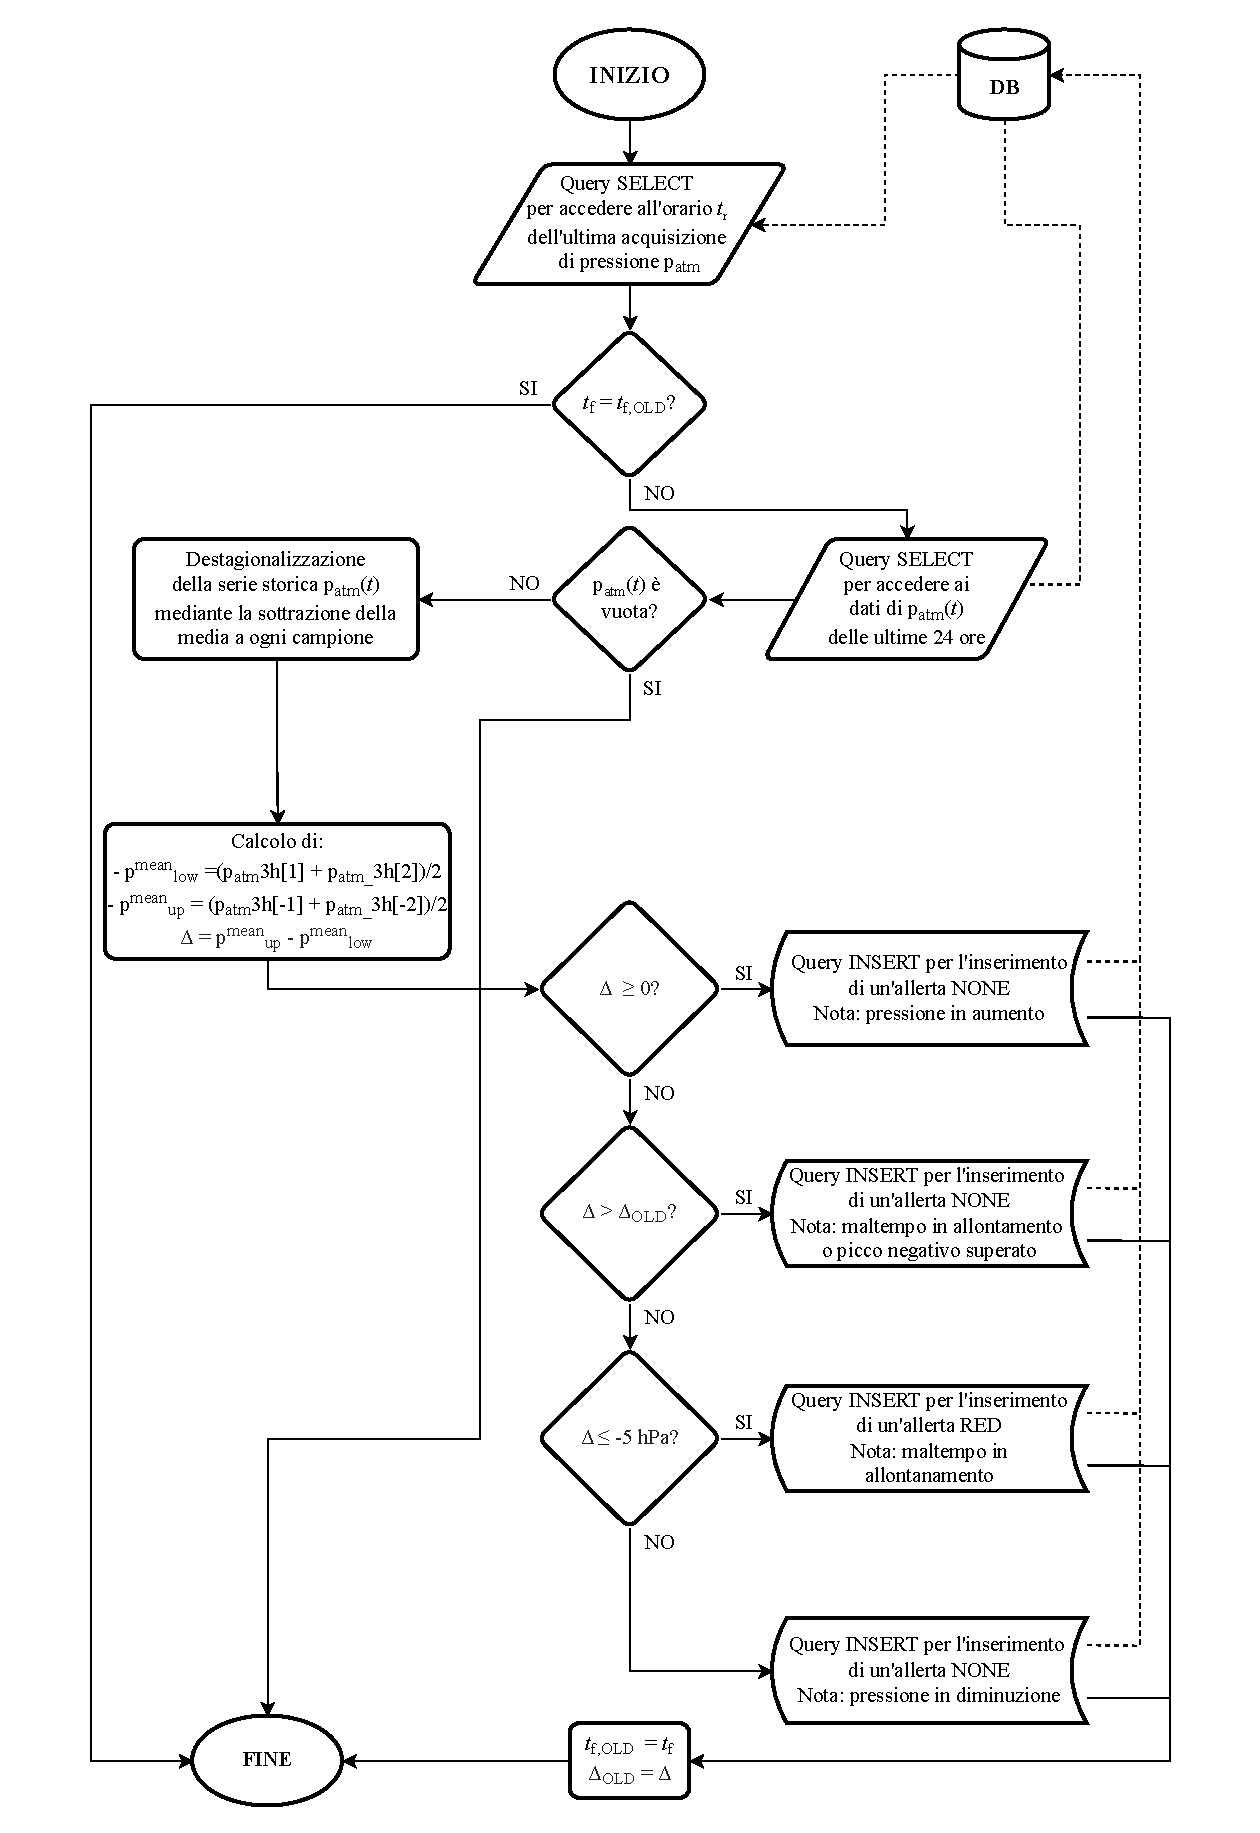
\includegraphics[height=590px]{./Iterazione 3/OtherFiles/FC - Generatore allerte BW.pdf}
	\caption{diagramma di flusso relativo all'algoritmo di generazione delle allerte maltempo.}
	\label{fig:BFFlowChart}
\end{figure}

\clearpage

\paragraph{Generatore di allerte nebbia e brina}

\subparagraph{Cenni di meteorologia} Per prevedere le formazioni di nebbia e brina è necessario calcolare il \textit{punto di rugiada} T$_d$, ossia la temperatura alla quale l'acqua contenuta nell'aria di un ambiente condensa e si trasforma in gocce d'acqua; esso viene raggiunto quando l'umidità relativa raggiunge il \SI{100}{\percent}, cioè nell'istante in cui l'aria diventa satura e non riesce più a contenere l'umidità ambientale. Il punto di rugiada si determina tramite l'\textit{approssimazione di Magnus-Tetens}:
\[ T_d = \frac{b \cdot \alpha(T,UR)}{a - \alpha(T,UR)}\]
\[\mbox{con } \alpha(T,UR) = \frac{a \cdot T}{b + T} + \ln(UR) \mbox{, } a = \si{17,27} \mbox{ e } b = \si{237,7}\si{\degreeCelsius}\]
\[T\mbox{ (temperatura misurata): } \SI{-20}{\degreeCelsius} < T < \SI{60}{\degreeCelsius}\]
\[UR\mbox{ (umidità relativa): } 0,01 < UR < 1,00\]
La nebbia si forma quando T = T$_d$, mentre la brina quando T = T$_d$ con T$_d < 0$

\subparagraph{Descrizione dell'algoritmo} Per generare le allerte nebbia e brina si deve calcolare la temperatura di rugiada T$_d$ (o \textit{dew point}), la quale a sua volta è funzione della temperatura T e dell'umidità relativa UR. Pertanto, dopo aver verificato la diversità tra $t_f$ e $t_{f,OLD}$, il primo passo dell'algoritmo (figura \ref{fig:FFFlowChart1}), viene eseguita una query per accedere ai dati di temperatura delle ultime 24 ore rilevati dalla stazione APRS.FI associata alla zona di competenza del thread. Questo parametro atmosferico dev'essere studiato tramite un modello statistico affinché possa essere previsto il suo comportamento nel breve termine; la scelta è ricaduta sull'ARIMA, un modello ARMA che rende stazionaria, se già non lo fosse, la serie storica tramite differenziazioni. Per identificare il modello, ossia per stimare il valore dei suoi parametri a massima verosimiglianza (o MLE), e per svolgere l'analisi di complessità, una procedura basata sulla minimizzazione dell'informazione di Akaike (o AIC), è stata utilizzata la funzione \textit{auto\_arima} del package \textit{pmdarima} disponibile per il linguaggio Python. Da notare che a ogni iterazione viene stimato un nuovo modello utilizzando anche l'acquisizione più recente presente nel DB. Una volta conclusa l'operazione di stima dell'ARIMA, esso viene impiegato per svolgere una predizione a 3 passi della temperatura, ossia a:
\begin{itemize}
	\item $t_1 = t_f + k$; 
	\item $t_2 = t_f + 2 \cdot k$;
	\item $t_3 = t_f + 3 \cdot k$; 
\end{itemize}
con \textit{k} che rappresenta il tempo che intercorre tra due rilevazioni consecutive da parte della stazione meteorologica (circa \SI{10}{\minute}) e $t_f$ la data e l'ora dell'acquisizione più recente presente nel DB. Lo stesso studio a scopo predittivo viene fatto anche per l'umidità relativa. Una volta note le previsioni di T e UR, esse vengono combinate per fare la predizione a 3 passi della temperatura di rugiada T$_d$. Dopodiché, vengono calcolati gli intervalli di validità I, IC$_1$, IC$_2$ e IC$_3$ entro i quali la temperatura deve rientrare affinché venga generata un'allerta. Essi sono necessari non solo perché mai si otterrà un'uguaglianza tra T(\textit{t}) e T$_d$(\textit{t}) a causa degli errori di predizione, ma anche perché la condensazione dell'acqua contenuta nell'aria può avvenire a una temperatura superiore a quella di rugiada; T$_d$, infatti, non tiene conto nè della temperatura del suolo, il quale potrebbe essere più freddo della colonna d'aria che lo sovrasta, nè della presenza di sostanze chimiche capaci di alterare il dew point. Gli intervalli sono asimmetrici poiché T non può essere più piccola di T$_d$; se così fosse l'umidità relativa supererebbe il \SI{100}{\percent}, un evento fisicamente impossibile. Per i criteri di generazione delle allerte si invita a visualizzare la figura \ref{fig:FFFlowChart2}; si noti che l'allerta brina viene creata quando la temperatura, attuale $T(t_f)$ o prevista $\hat{T}(t_1|t_f)$, $\hat{T}(t_2|t_f)$ e $\hat{T}(t_3|t_f)$: 
\begin{itemize}
	\item rientra nel proprio intervallo di validità (es. $\hat{T}(t_1|t_f) \in$ IC$_1$ $= [\hat{T_d}(t_1|t_f);\hat{T_d}(t_1|t_f) + \SI{0.45}{\degreeCelsius}]$);
	\item è non-positiva (es. $\hat{T}(t_1|t_f) \le 0$).
\end{itemize} L'algoritmo, infine, termina con l'aggiornamento di $t_{f,OLD}$.        

\begin{figure}[h!]
	\centering
	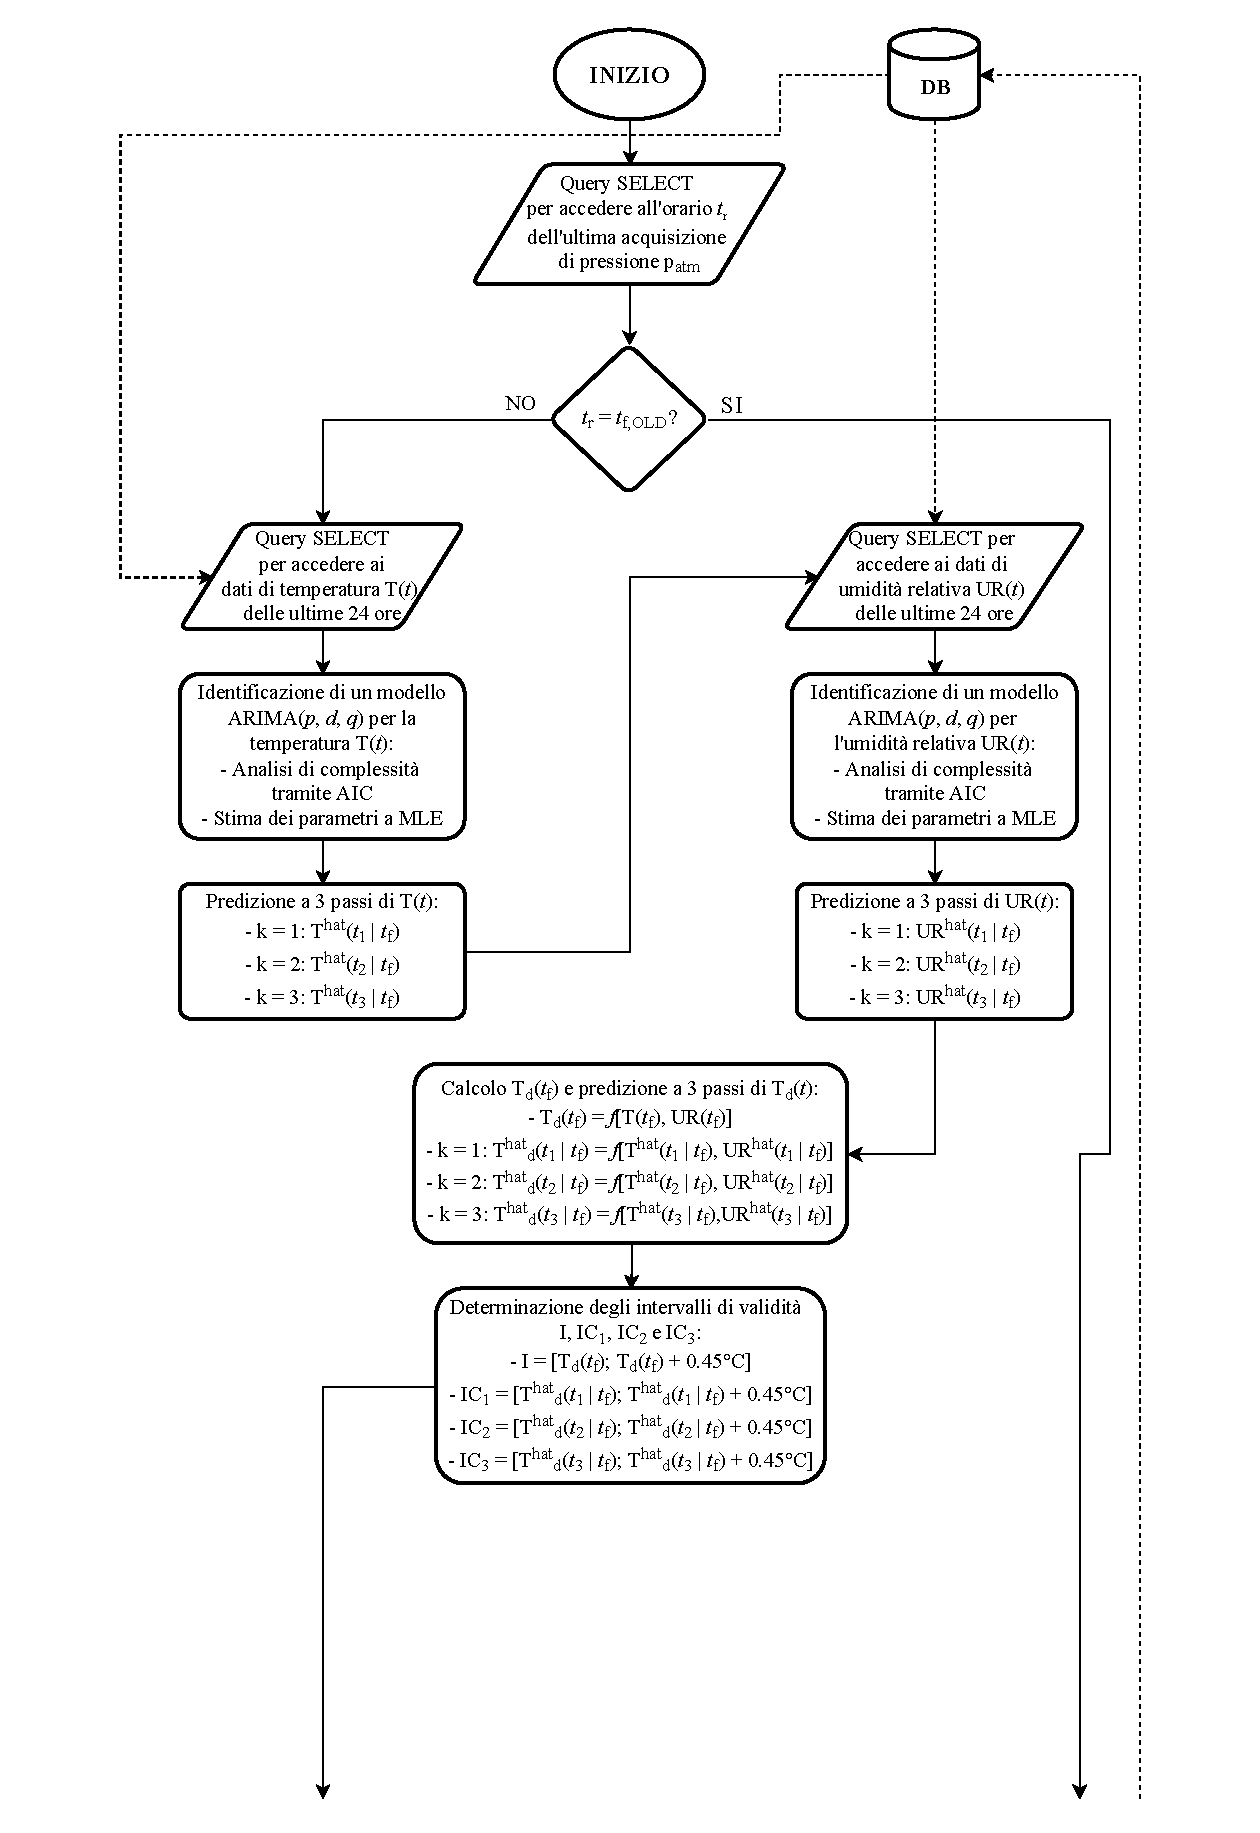
\includegraphics[height=590px]{./Iterazione 3/OtherFiles/FC - Generatore allerte F&F(1).pdf}
	\caption{Diagramma di flusso relativo all'algoritmo di generazione delle allerte nebbia e brina, prima parte.}
	\label{fig:FFFlowChart1}
\end{figure}

\begin{figure}[h!]
	\centering
	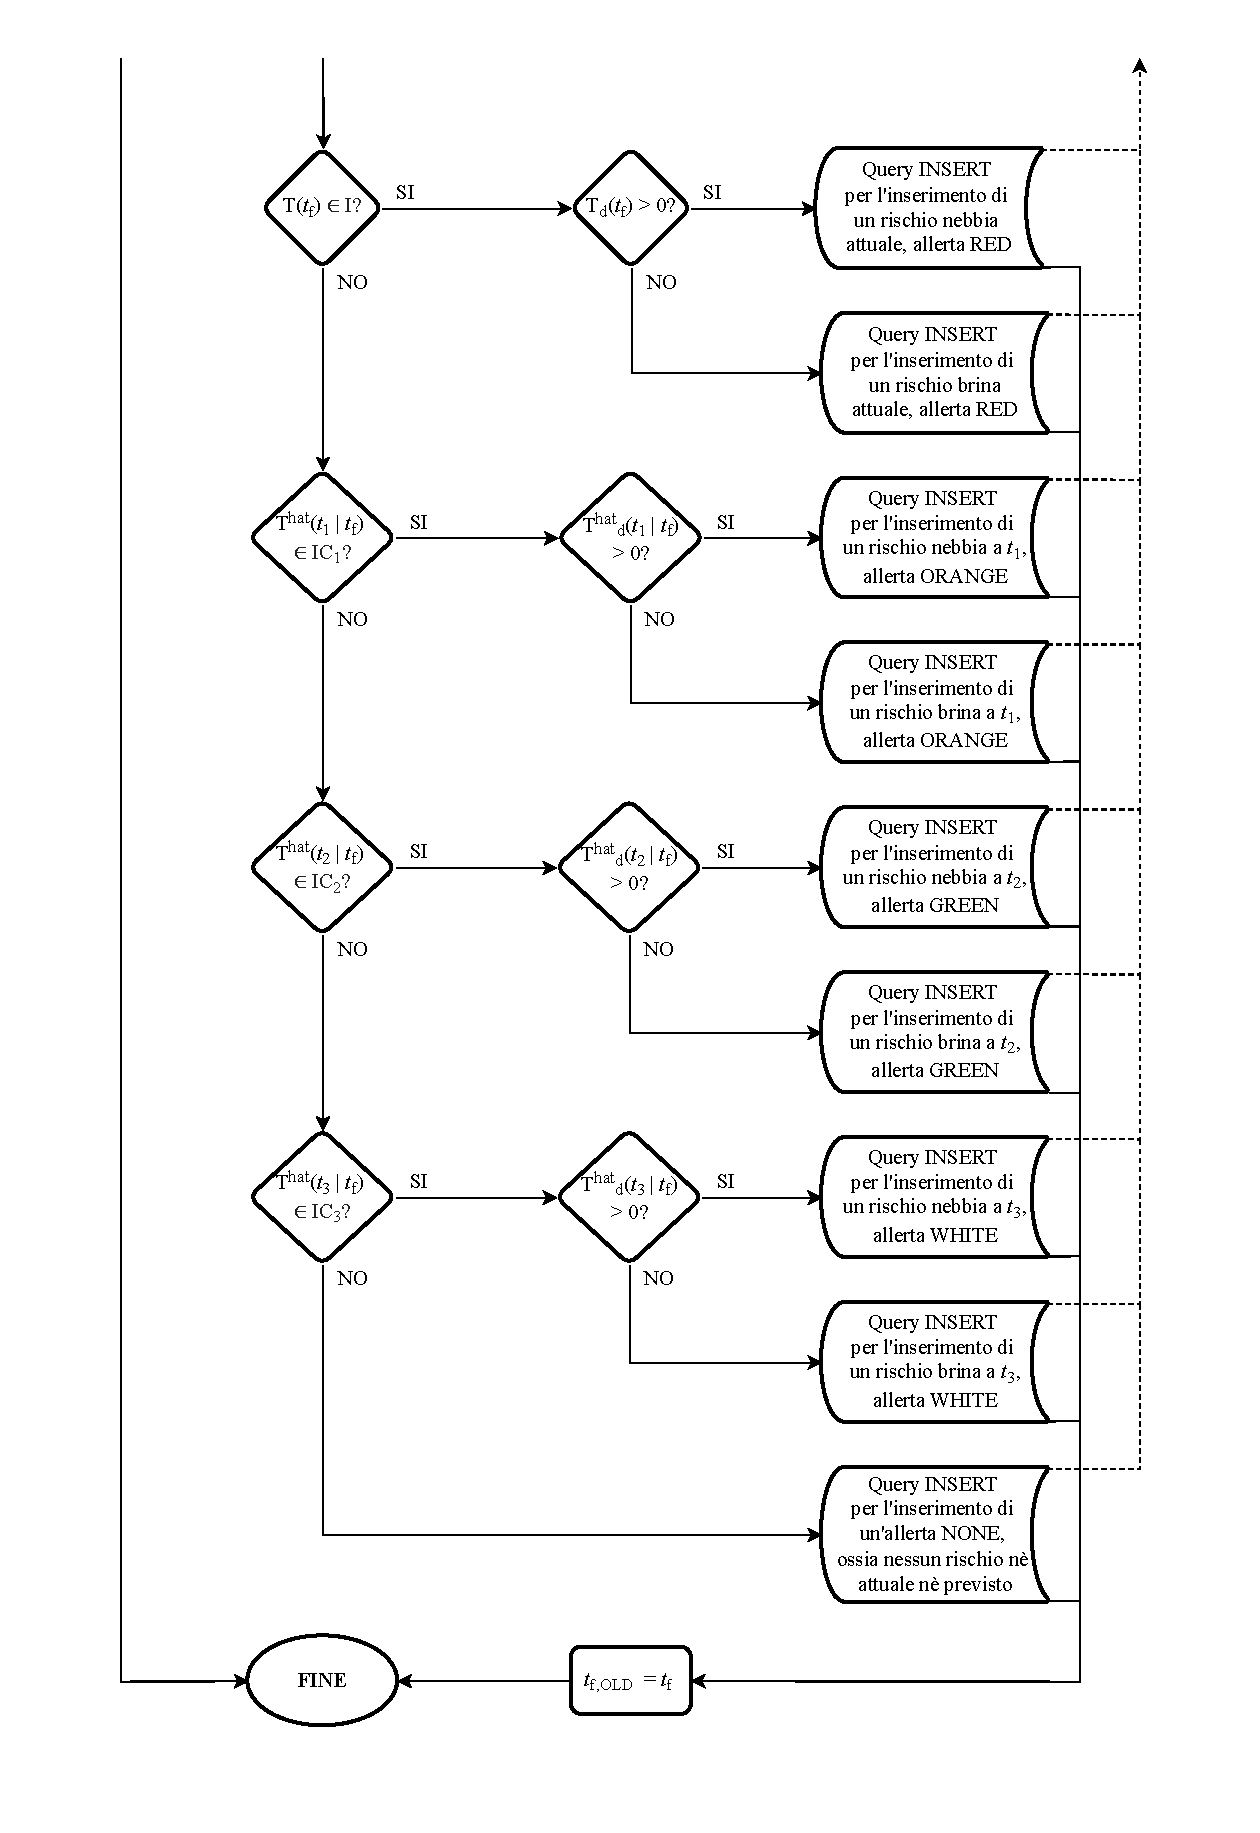
\includegraphics[height=590px]{./Iterazione 3/OtherFiles/FC - Generatore allerte F&F(2).pdf}
	\caption{Diagramma di flusso relativo all'algoritmo di generazione delle allerte nebbia e brina, seconda parte.}
	\label{fig:FFFlowChart2}
\end{figure}

\clearpage

\paragraph{Algoritmo}

\SetKwComment{Comment}{/* }{ */}
\RestyleAlgo{ruled}
\begin{algorithm}
	\caption{Data Analyzer}
	\SetKwProg{Al}{algoritmo}{ is}{end}
	\Al{generateAlarms($area\_DS$, $num\_areas$)}{
		\textbf{/* Avvio dei generatori di allerte */}\;
		\For{$i = 1$ \KwTo $num\_areas$}{
			\underline{badWeatherAlertsCreator}($area\_DS$ [$i$ ; `nameAprStation'], $area\_DS$[$i$ ; `idArea'], $i$, $old\_final\_time\_list$, $old\_delta\_list$)\;
			\underline{fogFrostAlertsCreator}($area\_DS$ [$i$ ; `nameAprStation'], $area\_DS$[$i$ ; `idArea'], $i$, $old\_final\_time\_list$)\;
		}
	}
\label{alg:1}

\end{algorithm}

\begin{algorithm}
	\SetKwProg{Fn}{function}{ is}{end}
	\SetKwProg{Class}{Class}{:}{end}
	\SetKwIF{If}{ElseIf}{Else}{if}{then}{else if}{else}{end}
	\caption{generatore di allerte maltempo}
	\Fn{badWeatherAlertsCreator(station\_code, areaID, index, old\_final\_time\_list, old\_delta\_list)}{
		$recent\_time \gets$ data ultima acquisizione della stazione $station\_code$\;
		\textbf{/* Interruzione della funzione se non ci fosse una nuova acquisizione */}\;
		\If{$recent\_time = old\_final\_time\_list\left[index\right]$}{
			\textbf{exit}\;
		}
		\textbf{/* Elaborazione della serie storica relativa alla pressione atmosferica */}\;
		$pressure\_DS\gets$ recupera i dati di pressione atmosferica delle ultime \num{24} ore della stazione $station\_code$\;
		\If{$parameter\_DS$ is empty}{\textbf{exit}\;}
		$p\_mean \gets$ mean($pressure\_DS$[all ; `pressure'])\;
		\For{$i = 1$ \KwTo lenght($pressure\_DS$)}{
			$pressure\_DS$[$i$] $\gets pressure\_DS$[$i$] - $p\_mean$ \Comment*[r]{Destagionalizzazione} 
		}
		$pressure\_DS \gets$ seleziona pressione ultime \num{3} ore\;
		$p\_low \gets$ mean($pressure\_DS$[\num{1}:\num{2}])\;
		$p\_up \gets$ mean($pressure\_DS$[end-\num{1}:end])\;
		$delta \gets p\_up - p\_low$\;
		\textbf{/* Generazione delle allerte relative al maltempo */}\;
		\uIf{$delta \ge 0$}{
			crea un'allerta NONE, pressione in aumento\;
			inserisci l'allerta nel DB\;
		}
		\uElseIf{$delta > old\_delta\_list\left[index\right]$}{
			crea un'allerta NONE, maltempo in allontanamento\;
			inserisci tramite una query l'allerta nel DB\;
		}
		\uElseIf{$delta < -\SI{5}{\hecto\pascal}$}{
			crea un'allerta RED, maltempo in avvicinamento\textbackslash picco negativo superato\;
			inserisci l'allerta nel DB\;
		}
		\Else{
			crea un'allerta NONE, pressione in diminuzione\;
			inserisci l'allerta nel DB\;
		}
		\textbf{/* Aggiornamento delle strutture dati di supporto */}\;
		$old\_final\_time\_list \left[index\right] \gets recent\_time$\;
		$old\_delta\_list\left[index\right] \gets delta$\;
	}
\label{alg:2}
\end{algorithm}

\begin{algorithm}
	\SetKwProg{Fn}{function}{ is}{end}
	\SetKwIF{If}{ElseIf}{Else}{if}{then}{else if}{else}{end}
	\caption{generatore di allerte nebbia e brina, parte 1}
	\Fn{fogFrostAlertsCreator(station\_code, areaID, index, old\_final\_time\_list)}{
		$recent\_time \gets$ data ultima acquisizione della stazione $station\_code$\;
		\textbf{/* Interruzione della funzione se non ci fosse una nuova acquisizione */}\;
		\If{$recent\_time = old\_final\_time\_list\left[index\right]$}{
			\textbf{exit}\;
		}
		\textbf{/* Predizione dei valori di temperatura e umidità relativa */}\;
		$summaryT \gets$ crea una tabella per la temperatura con colonne \{`I\_low', `value', `I\_up'\} e righe \{`tf', `t1', `t2', `t3'\}\;
		$summaryUR \gets$ crea una tabella per l'umidità relativa con colonne \{`I\_low', `value', `I\_up'\} e righe \{`tf', `t1', `t2', `t3'\}\;
		$summaryTd \gets$ crea una tabella per la temperatura di rugiada con colonne  \{`I\_low', `value', `I\_up'\} e righe \{`tf', `t1', `t2', `t3'\}\;
		\underline{tempURForcaster}(`temperature',$station\_code$, $summaryT$)\;
		\underline{tempURForcaster}(`umidity', $station\_code$, $summaryUR$)\;
		\textbf{/* Calcolo dei valori attuali e previsti della temperatura di rugiada */}\;

		\For{$i$ \KwTo $summaryTd.rows$}{
			$summaryTd$[$i$ ; `value'] $\gets$ calcolo temperatura di rugiada usando $summaryT$[$i$,`value'] e $summaryUR$[$i$,`value']\;
			$summaryTd$[$i$ ; `I\_up'] $\gets$ $summaryTd$[$i$ ; `value'] + \num{0.45}\;
			$summaryTd$[$i$ ; `I\_low'] $\gets$ $summaryTd$[$i$ ; `value']\;
		}
		\textbf{/* Generazione delle allerte nebbia e brina */}\;
		\underline{alertsCreator}($summaryT$, $summaryTd$)\;
		$old\_final\_time\_list \left[index\right] \gets recent\_time$\;
	}
\end{algorithm}

\begin{algorithm}
	\SetKwProg{Fn}{function}{ is}{end}
	\SetKwIF{If}{ElseIf}{Else}{if}{then}{else if}{else}{end}
	\caption{generatore di allerte nebbia e brina, parte 2}
	\Fn{tempURForcaster(parameter, station\_code, dataToUpdate)}{
		\eIf{$parameter$ = `temperature'}{
			$parameter\_DS \gets$ recupera dati di temperatura delle ultime \num{24} della stazione $station\_code$\;
		}{
			$parameter\_DS \gets$ recupera dati di umidità delle ultime \num{24} della stazione $station\_code$\;
		}
		
		\If{$parameter\_DS$ is empty}{\textbf{exit}\;}
		
		\textbf{/* Analisi dei dati */}\;
		$model \gets$ fitARIMA($parameter\_DS$[all ; $parameter$], $start\_complexity$ = [\num{1}, \num{1}, \num{1}], $stop\_complexity$ = [\num{3}, \num{3}, \num{3}]) \Comment*[r]{Stima del modello ARIMA}
		$k \gets$ \num{3} \Comment*[r]{Passo della predizione}
		$\left[fc, confint \right] \gets$ predict($model$, $k$) \Comment*[r]{Predizione a $k$ passi}
		\textbf{/* Aggiornamento del dataset */}\;
		$dataToUpdate$[`tf' ; all] $\gets$ $parameter\_DS$[end ; $parameter$]\;
	
		\For{$i$ = 1 to k}{
			$dataToUpdate[$i$,'value'] \gets$ fc[i]\;
			$dataToUpdate[$i$,'I\_low'] \gets$ confint[i,'$ic\_low$']\;
			$dataToUpdate[$i$,'I\_up'] \gets$ confint[i, '$ic\_up$']\;
		}
	}
\end{algorithm}

\begin{algorithm}
	\SetKwProg{Fn}{function}{ is}{end}
	\SetKwIF{If}{ElseIf}{Else}{if}{then}{else if}{else}{end}
	\caption{generatore di allerte nebbia e brina, parte 3}
	\Fn{alertsCreator(summaryT, summaryTd)}{
		\uIf{$summaryTd$ ['tf' ; 'I\_low'] $ \le summaryT$[`tf' ; `value']$ \le summaryTd$ [`tf' ; `I\_up']}{
			\eIf{$summaryT$[`tf' ; `value'] $>0$}{
				crea un rischio nebbia attuale, allerta RED\;
				inserisci l'allerta nel DB\;	
			}{
				crea un rischio brina attuale, allerta RED\;
				inserisci l'allerta nel DB\;	
			}
		}

		\uElseIf{ $summaryTd$[`t1' ; `I\_low']$\le summaryT$[`t1' ; `value'] $\le summaryTd$[`t1' ; `I\_up']}{
			\eIf{$summaryT$[`t1' ; `value'] $>0$}{
				crea un rischio nebbia tra \SI{10}{\minute}, allerta ORANGE\;
				inserisci tramite una query l'allerta nel DB\;
			}{
				crea un rischio brina tra \SI{10}{\minute}, allerta ORANGE\;
				inserisci tramite una query l'allerta nel DB\;
			}	
		}
		\uElseIf{$summaryTd$[`t2' ; `I\_low']$ \le summaryT$[`t2' ; `value']$\le summaryTd$[`t2' ; `I\_up']}{
			\eIf{$summaryT$[`t2' ; `value'] $>0$}{
				crea un rischio nebbia tra \SI{20}{\minute}, allerta GREEN\;
				inserisci tramite una query l'allerta nel DB\;
			}{
				crea un rischio brina tra \SI{20}{\minute}, allerta GREEN\;
				inserisci tramite una query l'allerta nel DB\;
			}
		}
		\uElseIf{$summaryTd$[`t3' ; `I\_low']$\le summaryT$[`t3' ; `value']$\le summaryTd$[`t3' ; `I\_up']}{
			\eIf{$summaryT$[`t3' ; `value'] $>0$}{
				crea un rischio nebbia tra \SI{30}{\minute}, allerta WHITE\;
				inserisci tramite una query l'allerta nel DB\;
			}{
				crea un rischio brina tra \SI{30}{\minute}, allerta WHITE\;
				inserisci tramite una query l'allerta nel DB\;
			}	
		}
		\Else{
			crea un'allerta NONE, nessun rischio nè attuale nè previsto\;
			inserisci tramite una query l'allerta nel DB\;
		}
	}
\end{algorithm}

\clearpage

\paragraph{Analisi computazionale}
Procediamo ora con l'analisi della complessità temporale dell'algoritmo. L'algoritmo è composto da più funzioni. È importante notare che il parametro attorno a cui vogliamo studiare la complessità temporale è il numero di aree che viene passato come parametro alla funzione principale. Iniziamo l'analisi dalle funzioni più interne:

\begin{itemize}
	\item \textbf{badWheatherAlertsCreator}: questa funzione verifica se è in arrivo maltempo analizzando la pressione. È presente un ciclo for tramite cui viene effettuata la destagionalizzazione. Il ciclo for va da 1 a length(pressure\_DS). Tale parametro contiene i valori di pressione delle ultime 24 ore di una particolare stazione e, poichè un nuovo valore di pressione viene inserito nel database ogni 10 minuti, tale parametro è costante e di conseguenza anche la complessità del ciclo. Le restanti operazioni sono sequenze di if-else che, anche nel caso peggiore, hanno una complessità temporale costante.
	\item \textbf{tempURForcaster}: con questa funzione vengono eseguite la stima del modello ARIMA e la predizione a k passi. In questo caso è importante notare che il numero di parametri su cui vengono eseguite queste due operazioni è sempre lo stesso perchè vengono presi i dati delle ultime 24 ore, ed inoltre la stima del modello ARIMA ha una complessità limitata. C'è poi un ciclo for che va da 1 a k dove k è pari a 3. Di conseguenza, anche il costo di questa funzione è costante. 
	\item \textbf{alertsCreator}: questa funzione serve per inserire le allerte nebbia o brina nel database. Non sono presenti cicli, ma solo una sequenza di if-then-else che nel caso peggiore ha compunque una complessità costante.
	\item \textbf{generateAlarms}: è la funzione principale dell'algoritmo. All'interno della funzione è presente un unico ciclo che viene eseguito un numero di volte pari al numero di aree, \textit{num\_areas}. All'interno di questo ciclo vengono chiamate le funzioni analizzate in precedenza, le quali sono tutte costanti nel parametro \textit{num\_areas}. Di conseguenza, il costo computazionale di questa funzione è O(num\_areas) e dipende esclusivamente dal numero di aree di cui deve essere analizzata la presenza di allarmi.
\end{itemize}

\subsection{Test Data Analyzer}
Sono stati eseguiti anche dei test di unità sull'algoritmo. Nella figura \ref{fig:test_result_alg} sono riportano i risultati effettuati grazie al modulo di Python \texttt{unittest}. Si è testato la generazione dei seguenti allarmi:
\begin{itemize}
	\item allarme \textit{RED} per maltempo e allarme \textit{RED} per nebbia;
	\item allarme \textit{NONE} per maltempo e allarme \textit{RED} per brina;
	\item allarme \textit{NONE} per maltempo e allarme \textit{NONE} per nebbia;
	\item allarme \textit{NONE} per maltempo e allarme \textit{WHITE} per nebbia;
	\item allarme \textit{NONE} per maltempo e allarme \textit{GREEN} per nebbia.
\end{itemize}

\begin{figure}[h!]
	\centering
	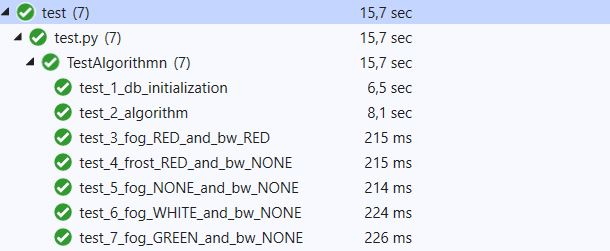
\includegraphics[width=1\linewidth]{./Iterazione 3/ImageFiles/TestResultAlgorithm}
	\caption{Risultati test algoritmo (interfaccia di Visual Studio).}
	\label{fig:test_result_alg}
\end{figure}

Di seguito è riportato il codice python relativo alla classe che implementa i test. Inizialmente, viene popolato un database di test con i dati caricati da dei file \textit{csv}. All'interno dei file è specificato il nome di una stazione APRS fittizia e i relativi dati di test di temperatura, umidità, pressione e data di acquisizione. Ogni test è associato a una diversa area.  Se le operazioni di caricamento termina correttamente, viene lanciata l'esecuzione dell'algoritmo. Se non si verificano eccezione, vengono poi controllati gli allarmi inseriti dall'algoritmo: se corrispondono agli allarmi attesi, il test è superato.

\begingroup
\UseRawInputEncoding
\lstinputlisting[language=python]{./Iterazione 3/OtherFiles/test_algorithm_script.py}
\endgroup

Inoltre, si riporta un esempio di allerta nebbia di tipo \textit{RED} generata dall'algoritmo il 6 febbraio 2022 (\Fig\ref{fig:test_previsione_alg}) sulla stazione meteorologica situata nei pressi della località di Ospitaletto (BS). Si è potuto verificare che questa allerta rispecchiasse veramente la situazione meteo attuale. Infatti, le previsioni meteorologiche attuali fornite da Google indicavano la presenza di nebbia (\Fig\ref{fig:test_previsione_google}).

\begin{figure}[h!]
	\centering
	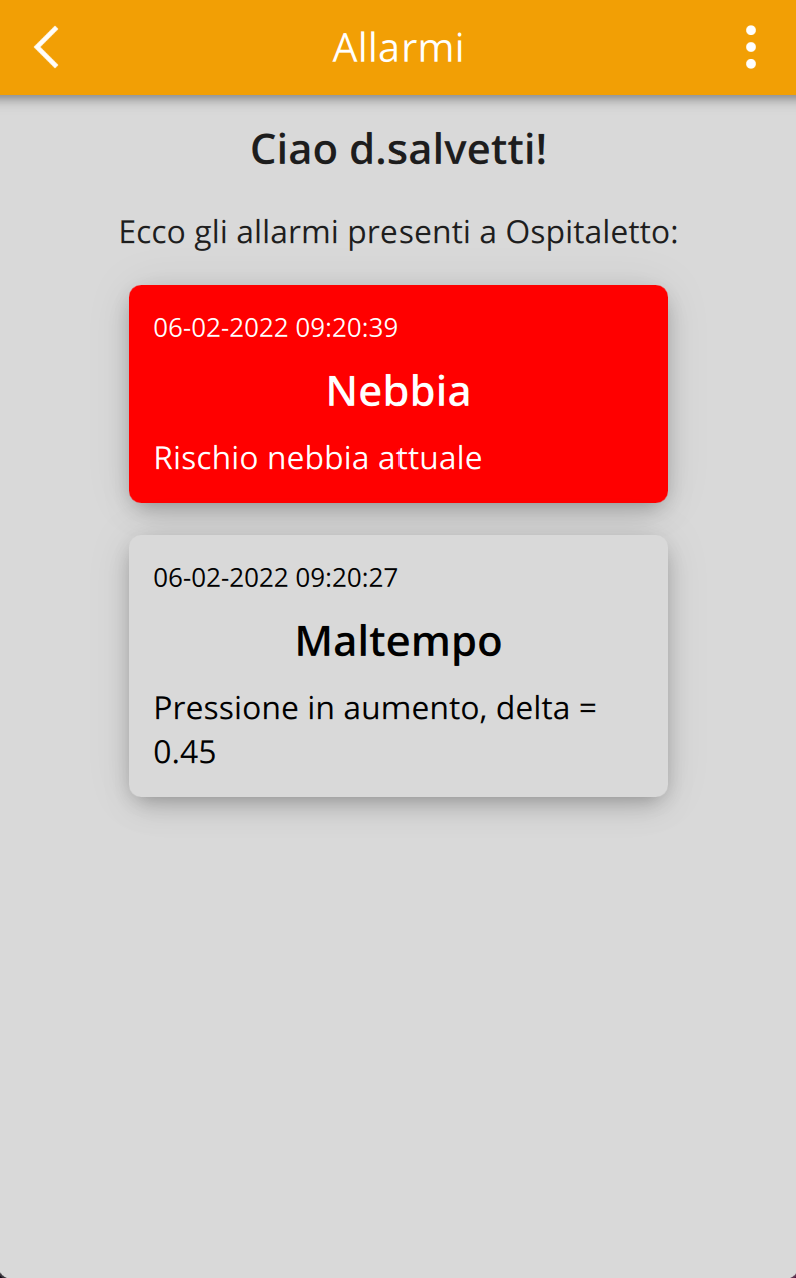
\includegraphics[width=0.3\linewidth]{./Iterazione 3/ImageFiles/testAppRedFog}
	\caption{Allarme nebbia attuale a Ospitaletto (BS) domenica 06/02/22 alle ore 9:20.}
	\label{fig:test_previsione_alg}
\end{figure}

\begin{figure}[h!]
	\centering
	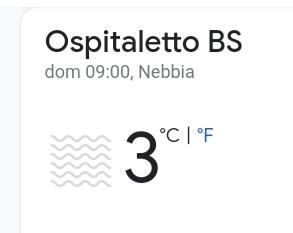
\includegraphics[width=0.2\linewidth]{./Iterazione 3/ImageFiles/Nebbia Ospitaletto Google}
	\caption{Meteo attuale fornito da Google a Ospitaletto (BS) domenica 06/02/22 alle ore 9:20.}
	\label{fig:test_previsione_google}
\end{figure}
